\documentclass[12pt]{beamer}

\usepackage[frenchb]{babel}
\usepackage[T1]{fontenc}
\usepackage[utf8x]{inputenc}    % accent
\usepackage{graphicx}           % pictures
\usepackage{multimedia}         % sounds and movies
\usetheme{Warsaw}
\title {Projet Picross}
\author{Groupe B}
\date{16 Mai 2014}
\institute{Université du Maine}



%%%%%%%%%%%%%%%%%
% PRÉAMBULE     %
%%%%%%%%%%%%%%%%%
\setbeamertemplate{itemize item}[circle]
\hypersetup{
        pdfpagemode = FullScreen,% afficher le pdf en plein écran
        pdfauthor   = {groupe B},%
        pdftitle    = {projet}%
        pdfsubject  = {projet},%
        pdfcreator  = {PDFLaTeX},%
}
\setbeamertemplate{navigation symbols}{
        \insertslidenavigationsymbol
        \insertframenavigationsymbol
        %\insertsubsectionnavigationsymbol
        %\insertsectionnavigationsymbol
        %\insertdocnavigationsymbol
        %\insertbackfindforwardnavigationsymbol
}
% Faire apparaître un sommaire avant chaque section
\AtBeginSection[]{
        \begin{frame}
        \begin{center}{\Large Plan }\end{center}
        %%% affiche en début de chaque section, les noms de sections et
        %%% noms de sous-sections de la section en cours.
        \tableofcontents[currentsection,hideothersubsections]
        \end{frame} 
}





%%%%%%%%%%%%%%%%%
% DOCUMENT      %
%%%%%%%%%%%%%%%%%
\begin{document}

\maketitle


% FRAME %%%%%%%%%%%%%%%%%%%%%%%%%%%%
\begin{frame}{}
  \tableofcontents
\end{frame}
   



%%%%%%%%%%%%%%%%%%
% Présentation
%%%%%%%%%%%%%%%%%%
\section{Présentation}


% FRAME %%%%%%%%%%%%%%%%%%%%%%%%%%%%
\begin{frame}{Présentation du Projet}
    \begin{enumerate}
      \item Presentation des membres
        \begin{enumerate}
        \item Lucas Bourneuf   (Chef de Projet)
        \item Ewen Cousin      (Developpeur GUI)
        \item Jaweed Parwany   (Developpeur Système)
        \item Charlie Marechal (Documentaliste)
        \item Nicolas Bourdin  (Developpeur GUI)
        \item Julien Legall    (Developpeur IA)
        \end{enumerate}\pause
      \item Objectif
        \begin{enumerate}
        \item  Créer un Picross en Ruby
        \end{enumerate}\pause
      \item Delai
        \begin{enumerate}
        \item 3 mois
        \end{enumerate}
    \end{enumerate}\pause
\end{frame}


\section{Realisation du Projet}
\subsection{Le déroulement du Projet}
\begin{frame}{Réalisation du Projet}
 %\begin{enumerate}
  %\item Le déroulement du Projet
    %\begin{enumerate}
    %\item Diagramme de Gantt
    %\item  Diagramme UML
    %\end{enumerate}
     %\end{enumerate}
\end{frame}
\begin{frame}
  %{Diagramme de Gantt}
  %\begin{figure}[t]
    %\centering
    %\includegraphics[height=\dimexpr11\textheight/16\relax]{ganttDiagramm}
    %\caption{Diagramme de Gantt}
  %\end{figure}
\end{frame}
\begin{frame}
  %{Diagramme de UML}
  %\begin{figure}[t]
    %\centering
    %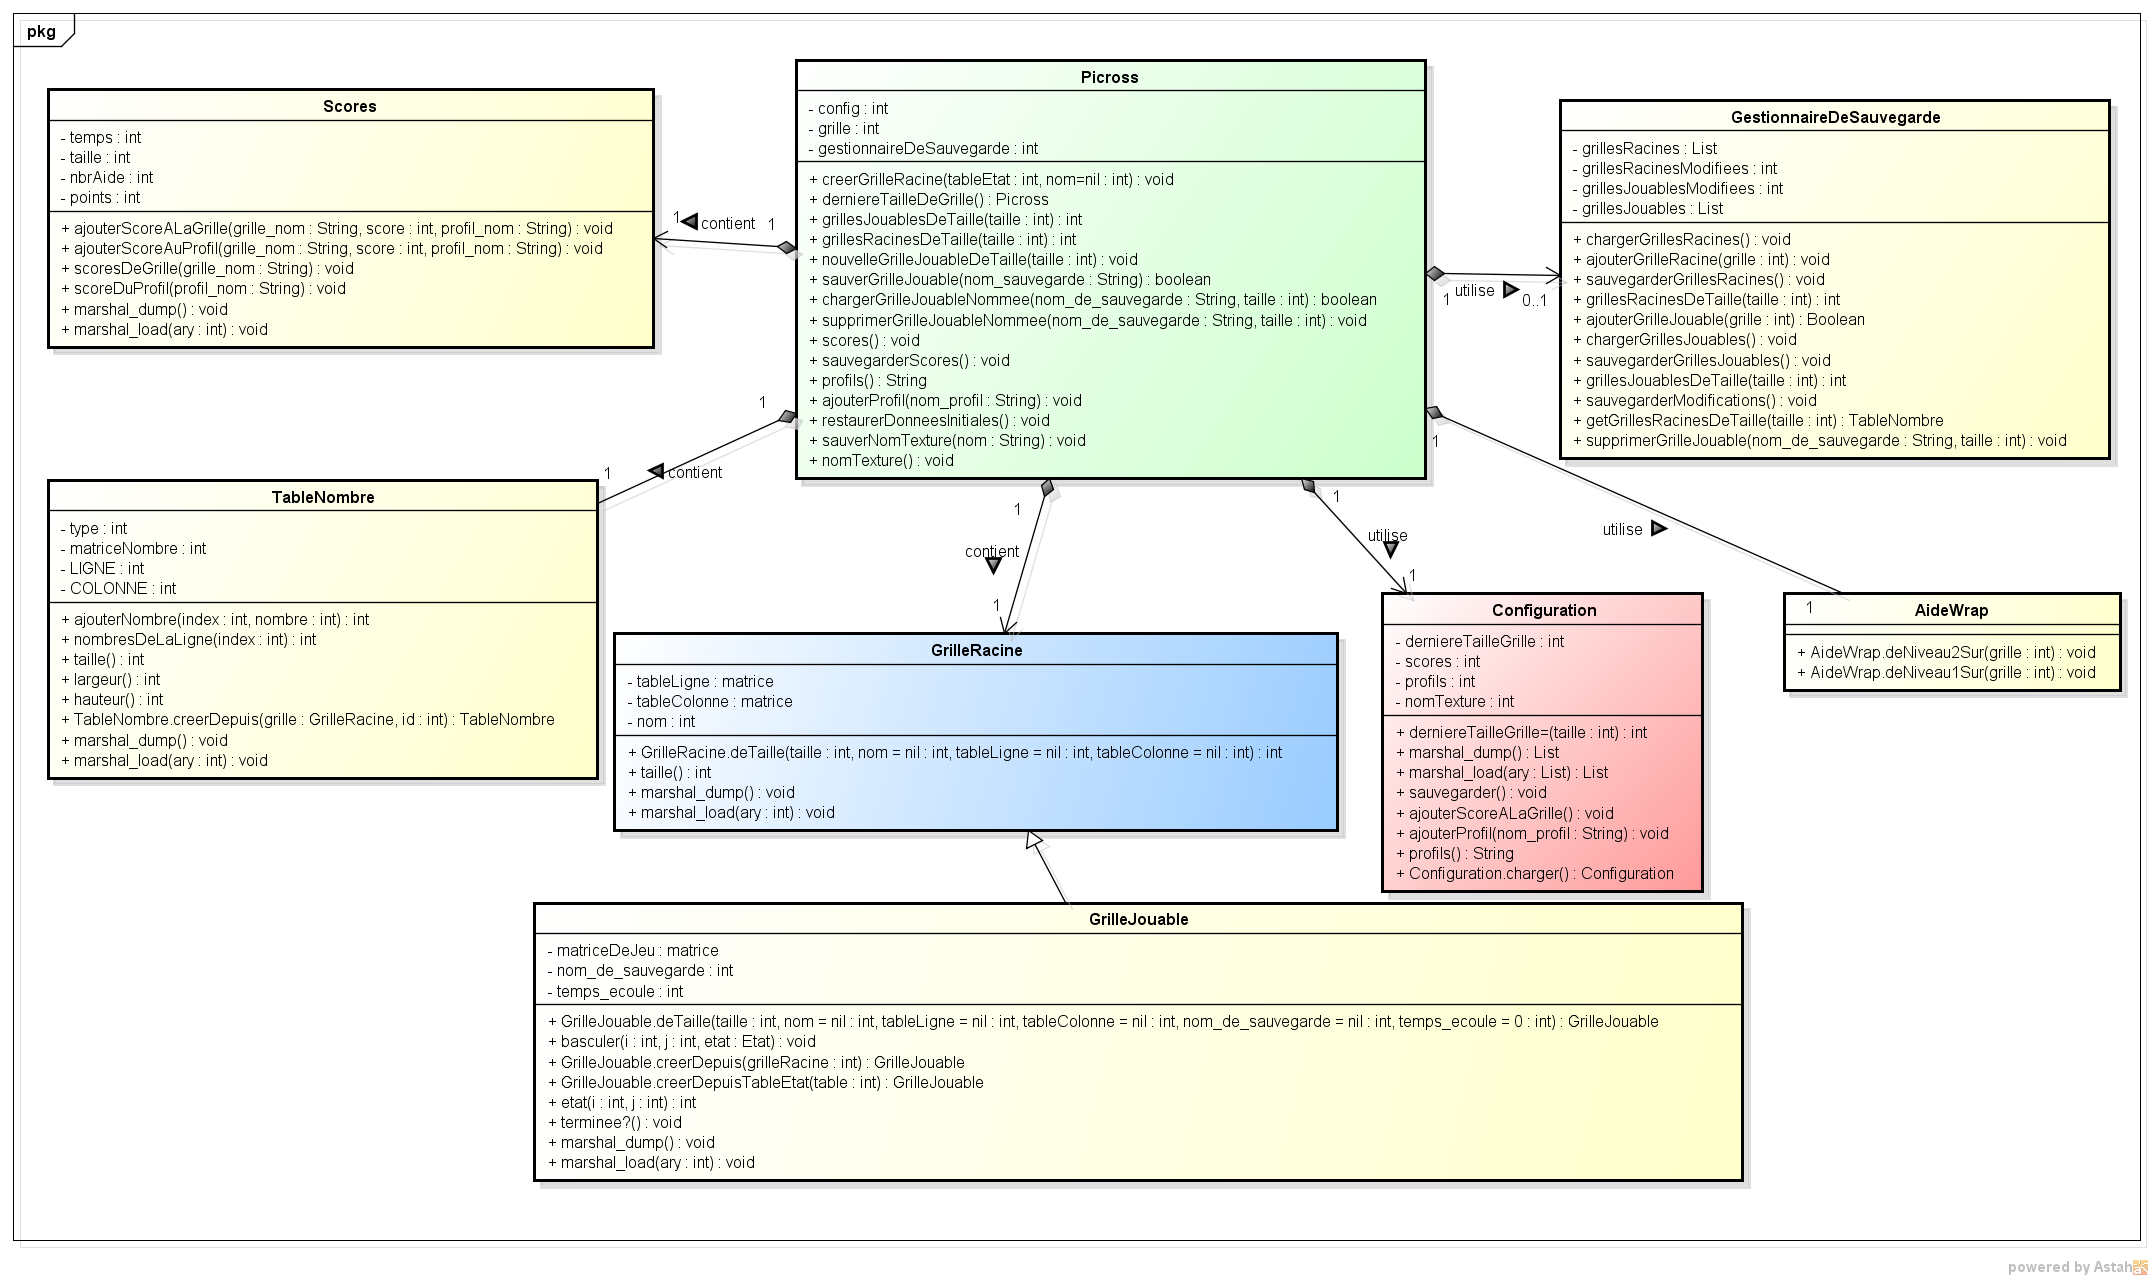
\includegraphics[height=\dimexpr11\textheight/16\relax]{UMLDiagram}
    %\caption{Diagrammes UML}
  %\end{figure}
\end{frame}


 \subsection{Fonctionalité}
    \begin{frame} {Fonctionalité}
     %\begin{enumerate}
     
      %\item Fonctionalité
        %\begin{enumerate}
            %\item l'aide
               %\begin{enumerate}
                    %\item En cas de blockage on peut avoir accés à l'aide 
                    %\item Permet de trouver une solution 
                %\end{enumerate}\pause
            %\item gestion de sauvegarde
                %\begin{enumerate}
                    %\item Sauvegarde la partie dans un fichier
                %\end{enumerate}\pause
            %\item score
                %\begin{enumerate}
                    %\item Affiche le score du joueur 
                %\end{enumerate}
         %\end{enumerate}\pause
        %\end{frame}

         %\item Probléme rencontré
            %\begin{enumerate}
                %\item gestion du score 
            %\end{enumerate}
          %\end{enumerate}\pause
        \end{frame}

\subsection{Aspects techniques}
    \begin{frame}
        \begin{enumerate}
            \item Languages
                \begin{itemize}
                    \item Ruby 
                \end{itemize}
            \item Support   
            \begin{enumerate}
                \item Environnement Unix
            \end{enumerate}
        \end{enumerate}
    \end{frame}

\subsection{Outils}
    \begin{frame}
        \begin{enumerate}
           \item Eclips IDE
       \end{enumerate}
    \end{frame}



\section{Conclusion}
\begin{frame}{Conclusion}
  
    %\begin{enumerate}
        %\item Presentation du travail
        %\begin{enumerate}
            %\item Bilan du projet 
        %\end{enumerate}\pause
        %\begin{enumerate}
            %\item Ce que l'on a appris
            %\begin{enumerate}
                %\item Comment un projet se déroule
                %\item le travail collaboratif
            %\end{enumerate}
        %\end{enumerate}
    %\end{enumerate}\pause
\end{frame}
\appendix[Questions ?]
\end{document}
